\section{Results and Discussion}

\subsection{Performance Analysis}
This chapter supplies some benchmarks, to analyze how close this thesis comes to achieve the wanted performance, which should be on eye level with C.

If not stated otherwise, benchmarks are written for this thesis and executed on an Intel Core i5-4200U with an HD 4400 graphic and 8GB of RAM.
Julia 0.4 has been used, C++ code hase been compiled with VS13 and for python the anaconda distribution with Python 2.7 was used.
Benchmarks were run on an idle computer with as little background processes running as possible.
The sources of the benchmarks can be found on Github.

\subsubsection{Julia}

Julia's performance is crucial for this thesis. 
If Julia does not perform close to C it would weaken the whole argument of writing the visualization library in Julia.
It is a very tedious task to write representative benchmarks for a programming language. 
The only way out is to rely on a multitude of sources and try to find analytical arguments.
In this thesis, Julia's own benchmark suite will be used in addition to some real world benchmarks.
In addition, the general compiler structure of Julia will be analyzed to find indicators for the limits of Julias performance.

\vspace{1em}
\begin{minipage}{\linewidth}
    \centering
    \includegraphics[width=0.9\linewidth]{graphics/juliabench.pdf}
    \captionof{figure}[Julia Performance]{Julia's performance compared to other languages, taken from Julia's micro bench suite \cite{JuliaBench}. Smaller is better, C performance = 1.0.}
    \label{fig:juliabench}
\end{minipage}

In the first benchmark from figure \ref{fig:juliabench}, we can see that Julia stays well within the range of C Speed. 
Actually, it even comes second to C-speed with no other language being that close.
This is a very promising first look at Julia, but it should be noted, that these benchmarks are written by the Julia core team.
So it is not guaranteed, that there is no bias favoring Julia in these benchmarks.
There is another benchmark comparing C++, Julia and F\#, which was created by Palladium Consulting which should not have any interest in favoring one of the languages.
They compare the performance of C++, Julia and F\# for an IBM/370 floating point to IEEE floating point conversion algorithm. This is part of a blog series\cite{JuliaFSCpp} written by Palladium Consulting.
F\# comes out last with 748.275 ms, than Julia with 483.769 ms and finally C++ with 463.474 ms. 
At the citation time, the Author had updated the C++ version to achieve 388.668 ms. 
It looks like the author was only working on making the C++ version faster, so it can not be said that the other versions could not have been made faster too.


The last Julia benchmark is more real world oriented. 
It is comparing Finite Element solver, which is an often used algorithm in material research and therefore represents a relevant use case for Julia.

\begin{table}[htbp]
    \centering
    \begin{tabular}{l|c|c|c}
        \hline
        \textbf{N}  & \textbf{Julia} & \textbf{FEniCS(Python + C++)}  & \textbf{FreeFem++(C++)}\\
        \hline
        121         & 0.99           & 0.67             & 0.01 \\
        2601        & 1.07           & 0.76             & 0.05 \\
        10201       & 1.37           & 1.00             & 0.23 \\
        40401       & 2.63           & 2.09             & 1.05 \\
        123201      & 6.29           & 5.88             & 4.03 \\
        251001      & 12.28          & 12.16            & 9.09 \\
        \hline
    \end{tabular}
    \captionof{table}[FEM Benchmark]{Performance of a FEM solver written in Julia compared to some existing libraries. \cite{FMSolver}}
    \label{table:fembench}
\end{table}
These are remarkable results, considering that the author states it was not a big effort to achieve this. After all, the other libraries are established FEM solvers written in C++, which should not be easy to compete with.

This list could go on, but it is more constructive to find out Julia's limits analytically.
As already mentioned, Julia is statically compiled at runtime. This means, as long as all types can be inferred at runtime, Julia will have in the most cases identical performance to C++.
The biggest remaining difference in this case is the garbage collection. Julia 0.3 has a mark and sweep garbage collector, while Julia 0.4 has an iterative mark and sweep garbage collector.
As seen in the benchmarks, it does not necessarily introduce big slowdowns.
But there are issues, where garbage collection introduces a significant slow down\cite{ReadDlmGC}.
Analysing this further is not in the scope of this thesis, though. 
But it can be said that Julia's garbage collector is very young and only the future will show how big the actual differences will be.

Another big difference is the difference in between different compiler technologies.
\ac{LLVM}'s biggest rival is \ac{gcc}. If C++ code that is compiled with \ac{gcc} is much faster than the same code compiled with \ac{LLVM}, the \ac{gcc} version will also be faster as a comparable Julia program.
In order to investigate the impact of this, one last benchmark will be analyzed.
This is a summary of a series of articles posted on Phoronix, which benchmarked \ac{gcc} 4.92 against \ac{LLVM} 3.5 and \ac{LLVM} 3.5 against \ac{LLVM} 3.6:
\begin{table}[ht]
  \centering
  \begin{tabular}{l|c|c}
    \hline
    \textbf{Method} & \textbf{\ac{gcc} vs \ac{LLVM} 3.5} & \textbf{\ac{LLVM} 3.5 vs \ac{LLVM} 3.6} \\
    \hline
    mean & 0.99 & 0.99 \\
    median & 0.97 & 1.00 \\
    maximum & 1.48 & 1.10 \\
    minimum & 0.39 & 0.88 \\
    \hline
  \end{tabular}
    \captionof{table}[gcc vs llvm summary]{Summary of the Phoronix benchmark. Unit is speedup of LLVM, bigger is better. \cite{LLVM35vsLLVM36}\cite{LLVMvsGCC}\cite{Phoronix}}
    \label{table:gccvsllvm}
\end{table}

The full tables can be found in the appendix under the table \ref{table:llvm35vsllvm36} and \ref{table:llvmvsgcc}.
The results suggest, that \ac{LLVM} is well in the range of \ac{gcc}, even though that there can be big differences between the two.
These are promising results, especially if you consider that LLVM is much younger than gcc. 
With big companies like Apple, Google\cite{GoogleAppleLLVM} and Microsoft\cite{MicrosoftLLVM} being invested in LLVM, it is to be expected that \ac{LLVM} will stay competitive, which means Julia should in theory stay competitive as well.


\subsubsection{ModernGL}
\vspace{1em}
\begin{minipage}{\linewidth}
    \centering
    \includegraphics[width=0.9\linewidth]{graphics/glbench.pdf}
    \captionof{figure}[OpenGL Wrapper]{Different performance of OpenGL wrappers. The time for $10^7$ calls was measured 100 times for each function.}
    \label{fig:openglwrapper}
\end{minipage}
\begin{table}[htbp]
    \centering
    \begin{tabular}{l|c|c|c}
        \hline
        \textbf{Function}   & \textbf{Python}    & \textbf{Staged Function} & \textbf{ModernGL} \\
        \hline
        glBindBuffer        & 64.43              & 1.00 & 1.04 \\
        glClearColor        & 474.72             & 1.02 & 1.04 \\
        glStringi           & 244.44             & 1.07 & 1.1  \\
    \end{tabular}
    \captionof{table}[OGL Relative Speed]{Performance relative to C++ with Glew (slowdown, bigger is worse)}
    \label{table:relativespeedoglw}
\end{table}

In this chapter, ModernGL, GLEW and PyOpenGL will get benchmarked.
The procedure was, to call an OpenGL function $10^7$ times in a tight loop. Execution time of the loop gets measured.
The results are plotted in figure \ref{fig:openglwrapper}.
ModernGL seems to do pretty well compared to C++ and python does very badly, with being up to 470 times slower in the case of glClearColor.
Julia in contrast offers nearly the same speed as calling OpenGL functions from C++ as can be seen in the table \ref{table:relativespeedoglw}.
As all the OpenGL wrappers are pretty mature by now and bind to the same C library (the video driver), this should mainly be a C function call benchmark.
Python performs badly here, but it must be noted that there are a lot of different Python distributions and some promise to have better C interoperability.
As this benchmarks goal is to show that Julia’s ccall interface is comparable to a C function call from inside C++, the python options have not been researched that thoroughly.
From this benchmark can be concluded, that Julia offers a solid basis for an OpenGL wrapper library.


\subsubsection{Reactive}

\begin{figure}
\centering
    \begin{minipage}{.5\textwidth}
        \centering
        \includegraphics[width=0.9\textwidth]{graphics/react_bench_2.pdf}
        \captionof{figure}[Reactive 1]{Complicated graph, simple calculation}
        \label{fig:reactive1}
    \end{minipage}%
    \begin{minipage}{.5\textwidth}
        \centering
        \includegraphics[width=0.9\textwidth]{graphics/react_bench_1.pdf}
        \captionof{figure}[Reactive 2]{High memory, simple event graph}
        \label{fig:reactive2}
    \end{minipage}
\end{figure}

It is relatively hard to benchmark the used event system in real world scenarious as it is hard to find a baseline.
One would have to rewrite Romeo with another Event system. 
Using other visulization libraries as a baseline is also difficult, as it is hard to isolate the performance of the event system.
This is why we will compare an event graph from Reactive with its unrolled version.
For the unrolled version the functions from the callback graph have been executed in the same order as the event graph would have without introducing any event system related overhead.
This way we can measure the overhead introduced by the event system.
Two code samples have been benchmarked, one simulating the operation needed for the camera and the other simulates animating a large array.
The first has low memory usage with a more complex event graph. The second has a straight forward event graph, but it must pass on a large array and needs to execute the callbacks on the array.

As can be seen in figure \ref{fig:reactive1}, small operations with a complex event graph has some noticable overhead. Reactive is in this scenario about 1.45 times slower than the optimal version.
This does not come as a surprise as sorting and managing the graph structure obviously adds some overhead.

The second scenario looks much better for Reactive. The performance difference is neglectable, making Reactive a good choice for creating signals with high memory throughput.

\subsubsection{3D Rendering Benchmark}

\begin{minipage}{\linewidth}
    \centering
    \includegraphics[width=\linewidth]{graphics/vispy_mayavi_romeo.jpg}
    \captionof{figure}[Benchmark]{Different visualizations of the same surface}
    \label{fig:reactive1}
\end{minipage}

The biggest problem with benchmarking the 3D rendering speed is, that there is no library which will allow to exactly reproduce similar conditions and measures. 
Additionally, without extensive knowledge of the library, it is difficult to foresee what gets benchmarked. 
As an example of why it is difficult to measure the frame rate we can look at Vispy. When you enable to measure the frame rate, it will show very low frame rates, as it only creates a new frame on demand.
On the other side Romeo has a fixed render loop, which renders as much frames as possible, leading to totally different amount of rendered frames per second. 
This is why it was decided, to use the threshold at which a similar 3D scene is still conceived as enjoyable and interactive. Usually the minimal amount of frames per second for perceiving movements as smooth is around 25.
So the benchmark was executed in the way, that the number regulating the complexity of the 3D scene was increased until one could not move the camera without stutters. The recorded threshold is than the result of the Benchmark.

First benchmark is an animated and still 3D surface plot. The libraries offering this functionality where Vispy, Mayavi and Matlab.

\begin{table}[htbp]
    \centering
    \begin{tabular}{l|l|l}
        \hline
        \textbf{Library} & \textbf{Still} & \textbf{Animated} \\
        \hline
        Vispy            & 300            & 80    \\
        Mayavi           & 800            & 150   \\
        Matlab           & 800            & 450   \\
        Romeo            & 900            & 600   \\
        \hline
        \hline
        Speed up Vispy   & 9x            & 56x   \\
        Speed up Mayavi  & 1.26x         & 16x   \\
        Speed up Matlab  & 1.26x         & 1.7x  \\
    \end{tabular}
    \captionof{table}[3D Benchmark]{3D surface created from a NxN matrix.}
    \label{table:relativespeedoglw}
\end{table}
Vispy had some issues, as the camera was never really smooth for the surface example. Also the normals were missing and there was no option to colorize the surface depending on the height.
It was decided to use the threshold of going from a little stutter to unpleasant stutters, making vispy not completely fail this benchmark.
For Vispy it was found out, that the normals where calculated on the CPU resulting in a major slow down\cite{VispyGithub}. The same can be expected for Mayavi, but Mayavi seems to be faster at calculating the normals.
There is not much information available on how Matlab renders their visualization, as it is closed source.

\begin{minipage}{\linewidth}
    \centering
    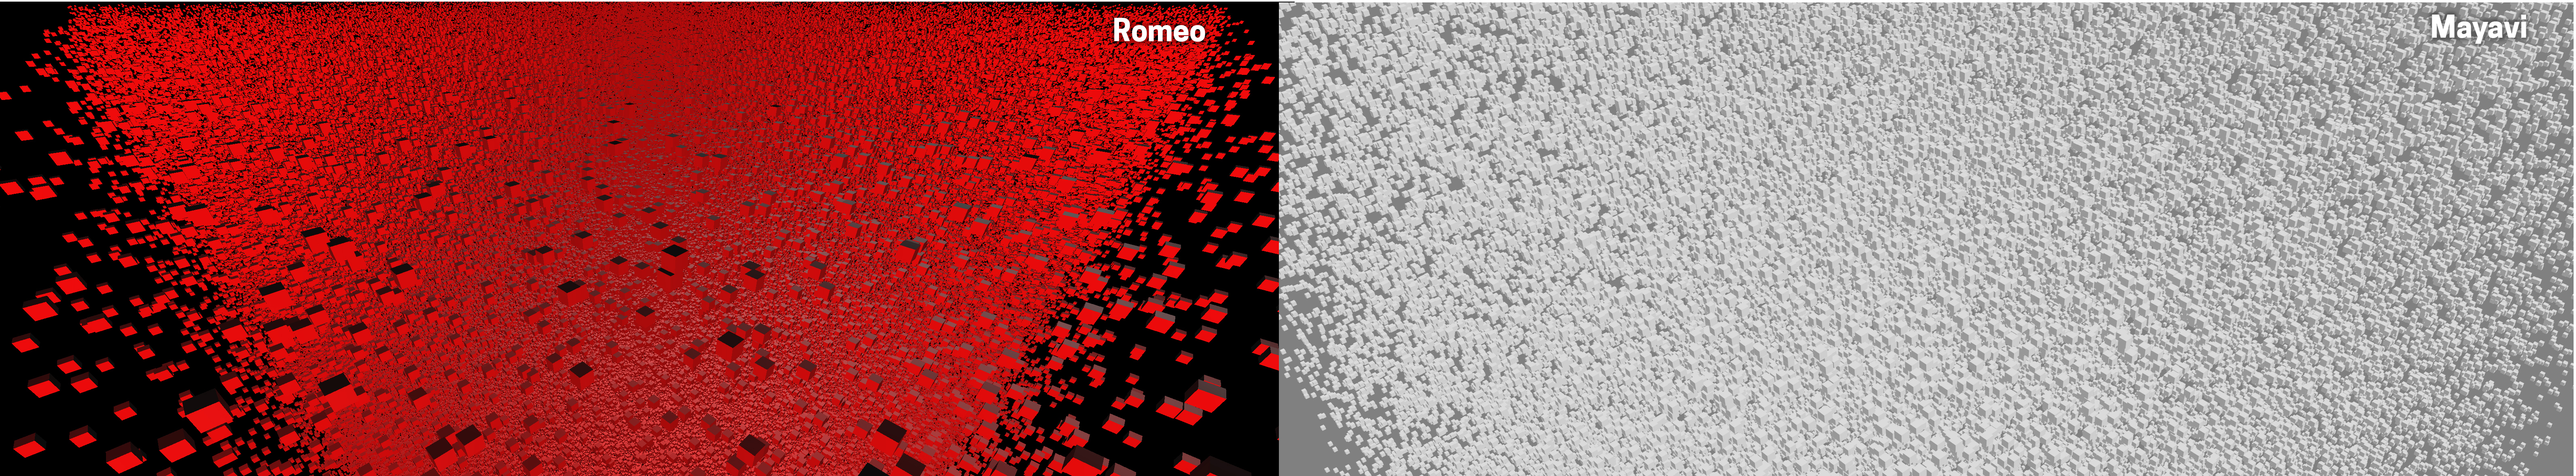
\includegraphics[width=\linewidth]{graphics/romeo_mayavi_particles.jpg}
    \captionof{figure}[Particles]{Rendered particles}
    \label{fig:reactive1}
\end{minipage}

The next benchmark is only between Romeo and Mayavi, as the other libraries did not offer a comparable solution. Matlab does not allow to use cubes as particle primitives and Vispy only had an example, where you needed to write your own shader, which can not be seen as a serious option. This is a benchmark for easy to use and high level plotting libraries. It is always possible to write an optimal version yourself in some framework, but what really interesting is, how well you can solve a problem with the tools the library has readily available.

\begin{table}[htbp]
    \centering
    \begin{tabular}{l|l|l}
        \hline
        \textbf{Library} & \textbf{Still}  & \textbf{Animated}  \\ 
        \hline
        Mayavi           & 90000           & 2500  \\
        Romeo            & 1000000         & 40000 \\
        \hline
        \hline
        Speed up         & 11x             & 16x \\
    \end{tabular}
    \captionof{table}[3D Benchmark]{Maximum number of particles that could be displayed without stutter.}
    \label{table:relativespeedoglw}
\end{table}
Romeo is an order of magnitude faster in this specific benchmark. This is most likely due to the fact that Romeo uses OpenGL's native instance rendering.


\subsubsection{IJulia}

It was not possible to compare IJulia directly with Romeo, as the feature set for plotting is too different.

But there are certain factors, which indicate, that is hard to reach optimal performance with IJulia.
First of all, IJulia uses ZMQ to bridge the web interface with the Julia kernel.
ZMQ is a messaging system using different sockets for communication like inproc, IPC, TCP, TIPC and multicas.
While it is very fast at it's task of sending messages, it can not compete with the native performance of staying inside one language.
This is not very important as long as there does not have to be much communication between Julia and the IPython kernel. This changes drastically for animations, where big memory chunks have to be streamed to the rendering engine of the browser. It can be expected, that this will always be a weakness of IJulia.
On the other hand, GPU accelerated rendering in a web browser is also limited.
It relies on WebGL, which offers only a subset of the OpenGL's functionality. So while the execution speed of OpenGL can be expected to be similar, there are a lot of new techniques missing, which can speed up rendering.

To investigate this another benchmark has been created.
It is between Romeo and Compse3D, which was the only library found to be able to display 3D models created with Julia directly from the IJulia notebook.
This benchmark is not entirely fair, as Compose3D is just a very rough prototype so far. 
But there seems to be no other library with which you can easily create and display interactive 3D graphics in the IJulia or IPython notebook. 
This benchmark creates a sierpinsky gasket and Compose3D displays it in the IJulia notebook while Romeo displays it natively in a window.

\begin{minipage}{\linewidth}
    \centering
    \includegraphics[width=\linewidth]{graphics/sierpinsky.jpg}
    \captionof{figure}[Sierpinsky]{Sierpinsky pyramid in 3D}
    \label{fig:reactive1}
\end{minipage}
\begin{table}[htbp]
    \centering
    \begin{tabular}{l|l}
        \hline
        \textbf{Library} & \textbf{Still}\\ 
        \hline
        Compose3D        & 15625         \\
        Romeo            & 1953125       \\
        \hline
        \hline
        Speed up         & 125x          \\
    \end{tabular}
    \captionof{table}[3D Benchmark]{Maximum number of pyramids that could be displayed without stutter.}
    \label{table:relativespeedoglw}
\end{table}

Again, Romeo is an order of magnitude faster. This can change in the future when Compose3D matures.
But one needs to notice, that Romeo utilizes OpenGL's instancing to gain this speed. Native instancing is not yet available in WebGL, which means that this optimization will not be available for the IPython notebook in the near future.

\subsection{Extensibility Analysis}

The modular design of Romeo has proven to be effective and the goal of re-usability has already proven itself.
Most of the created modules are used independently by different people.
GLVisualize is used by myself for two packages, namely GLPlot, a scientific plotting package for Julia and for a prototype of a file explorer.
It got forked by several users to create their own dynamic visualization packages.
The same applies for ModernGL and GLAbstraction. Most other used packages are at least used by one other project.
This indicates, that the abstraction and modularity is well designed, so that all the modules can function on their own.

The only exception is GLWindow, which has been used just indirectly through the other packages. 
This can mean three things.
First, it is badly abstracted and does not cleanly wrap one use case.
Secondly, it can be that the use case is not entirely clear to other people, which would not be a big surprise considering the minimal amount of documentation for GLWindow.
And finally, considering the small group of people developing graphics for Julia, it could be that they simply do not need the lower level functionality of GLWindow and instead rely on the other written packages that use GLWindow.

Modularity guarantees a broad user and developer base, which in turn results in rich functionality and stability.
From further analyzing the Github repository written for this thesis, one can find out that there is a general lack of documentation.
This hinders people from contributing and using the packages.

The implementation in just one language has been achieved by choice. There are only a few exceptions, like the kernel code for OpenGL shaders, which currently can not be written in Julia. 
Julia programmers that use Romeo can extend Romeo with Julia and immediately see their results without complicated compilations.
This together with the speed is one of the main achievements compared to other libraries offering similar functionality, like IJulia, Mayavi and Matlab.
To further proof this point I will analyze the mentioned software in more detail.
The language usage statistics and necessary tools needed in order to extend the software will be the main focus of the analysis.
One needs to note, that the usage statistic of languages is just a weak indicator for the extendability of a software.
Using different languages for one project can make sense if the project has different domains where domain specific languages give an advantage. As this means one needs to know all used languages, this still introduces complexity, but it is at least justified complexity.
This chapter will only discuss the complexity introduced by languages, which are only needed for compatibility with other libraries or because the main language is too slow. This is something, which should ideally be avoided.


\subsubsection{IJulia}

IJUlia is written in Julia and relies on ZMQ(C++) and IPython. 
IPython uses multiple JavaScript rendering back ends like Three.js and D3.
\begin{table}[htbp]
    \centering
    \begin{tabular}{l|l}
        \hline
        \textbf{Software} & \textbf{languages used}\\
        \hline
        IPython     & Python 78.5\% JavaScript:15.1\% HTML 5.0\% Other 1.4\%\\
        Three.js:   & JavaScript 62.4\% HTML 26.4\% Python 6.9\% C++ 1.9\% C 1.3\% GLSL 0.6\%\\
        D3:         & JavaScript 95.6\% CSS 4.3\%\\
        \hline
        \end{tabular}
    \captionof{table}[IJulia Stack]]{Technologies used in IJulia. Statistics taken from Github}
    \label{table:ijuliastack}
\end{table}
[more to come]

\subsubsection{Mayavi and VTK}

Table \ref{table:ParaviewStatistic} in the appendix shows an extensive summary of the used languages in the Paraview repository.
It amounts to a total of 3.642.105 lines of code written in 29 languages.
[more to come]

\subsubsection{Matlab}

Matlab is closed source, which makes the core of Matlab impossible to extend by the user.
This is why Matlab relays on a plug-in architecture, which enables developers to write closed or open source plug-ins for Matlab.
[Analysis of the plug-in Architecture]
[more to come]


\subsection{Usability Analysis}
%Consistency and ease of use of programming API in GLVisualize+GLAbstraction and Romeo.
%Short comment about the \ac{GUI}
Doing a broad user survey or similar methods was out of scope for this thesis.
As a result from this, the usability study has to be done analytically.
There are different aspects which can be analyzed. For example, how many function names need to be remembered, how easy they are memorized, if they expose the wanted functionality and how difficult it is to look up unknown functionality.
For this thesis, I will analyze the two main packages, namely GLVisualizes and GLAbstraction. 
The named aspects will be analyzed and in addition feedback from Github will be used.

GLVisulize has a very simple API, as it offers only five functions: visualize, visualizedefaults, edit and renderloop.
There are also the functions bounce and loop, which offers a simplification for creating periodic signals.
These functions might get moved into Reactive, though.
So for GLVisualize, only very few function names have to be remembered.
The question is, does this simple interface still allow people to create the visualization they want.
At closer inspection one can see, that visualize is overloaded 67 times, with each of these methods having a set of keyword arguments which enables further customization.
These can introduce drastic changes. The particle visualization for example can take any mesh as a primitive. This enables a customization, which was not possible in such an easy way in the other examined packages.
Also, most of the functions take either a data type, or a signal of that data type.
This makes it very intuitive to animate your data. 
In contrast, in order to setup the animation for the other packages, it took quite some time to find out how to update values of an existing visualization. This is acceptable, as it might take quite some time to find out that Romeo uses signals and how to work with signals.
But when this is found out, Romeo functions in the same, consistent way. Signals add a fourth dimension to any parameter or data you would like to visualize, making the usage principle consistent across the different visualizations.

For the other packages though, one needs to find out the names of the data for every visualization type in order to access and update them. Some attributes can not be animated, making the API even less consistent.

So for Romeo one can achieve anything by bringing the data into the right format.
Problems arise, if this can not be done easily or the format is not intuitive for the programmer.
To be fair, you will have this problem with every kind of visualization API. 
The difference is in the end, how easy it is to do the data transformations. 
Lets examine an example, where GLVisualize often will not allow to directly call visualize on the data.
There is only a method for visualizing a Mesh, but not for a vertex list plus a face list. If you work with mesh data, you will often handle the face and vertex list isolated.
So an API that offers a function like \texttt{visualize\_mesh(x::VertexList, y::FaceList)} will be more straightforward for a programmer.
Especially, as this is the standard way of displaying a mesh in most scientific plotting packages. This has become one of the most occurring questions on github, even though that there are usage examples for displaying a mesh.

But this functionality can be added in a simple way for GLVisualize by defining \texttt{visualize\_mesh(facelist, vertexlist) = visualize(Mesh(facelist, vertexlist))}.
As GLVisulize should stay as close to the principle of only having one function name, this should be moved to other interface only packages, though.
[more to come]